\documentclass[tikz, border=5pt]{standalone}

\begin{document}
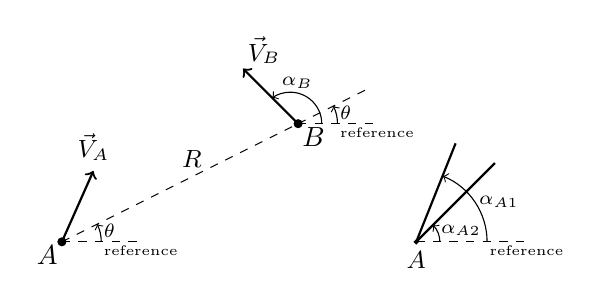
\begin{tikzpicture}

    %% Assignment-2

    % Collision diagram
    \begin{scope}
        % Mass A
        \coordinate (A) at (0,0);
        \draw[fill] (A) circle (0.05) node[below left=-2] {\( A \)};
        \draw[->, thick] (A) -- ++(0.4,0.9) node[above] {\small \( \vec{V}_A \)};

        % Mass B
        \coordinate (B) at (3,1.5);
        \draw[fill] (B) circle (0.05) node[below right=-2] {\( B \)};
        \draw[->, thick] (B) -- ++(-0.7,0.7) node[above right=-2] {\small \( \vec{V}_B \)};

        % Line of separation
        \draw[dashed] (A) -- (B) node[pos=0.55, above] {\small \( R \)};

        % Reference
        \draw[dashed] (A) -- ++(1,0) node[below=-2] {\tiny reference};
        \draw[dashed] (B) -- ++(1,0) node[below=-2] {\tiny reference};
        \draw[dashed] (B) -- ++(0.9,0.45);

        % Angles
        \draw[->] (A) ++(0.5,0) arc (0:27:0.5) node[pos=0.6, right=-2] {\scriptsize \( \theta \)};
        \draw[->] (B) ++(0.5,0) arc (0:27:0.5) node[pos=0.6, right=-2] {\scriptsize \( \theta \)};
        \draw[->] (B) ++(0.3,0) arc (0:125:0.4) node[above right] {\scriptsize \( \alpha_B \)};
    \end{scope}

    % Collision cone
    \begin{scope}[xshift=4.5cm, scale=0.5]
        \draw[fill] (0,0) circle [radius=0.05];
        \node[below] at (0,0) {\small \( A \)};

        % Lines
        \draw[dashed] (0,0) -- (2.8,0) node[below=-2] {\tiny reference};
        \draw[thick] (0,0) -- (2,2);
        \draw[thick] (0,0) -- (1,2.5);

        % Angles
        \draw[->] (0,0) ++(0.6,0) arc (0:45:0.6) node[pos=0.65, right=-2] {\scriptsize \( \alpha_{A 2} \)};
        \draw[->] (0,0) ++(1.8,0) arc (0:68:1.8) node[pos=0.5, right=-2] {\scriptsize \( \alpha_{A 1} \)};
    \end{scope}

\end{tikzpicture}
\end{document}
